\chapter{无穷复数项级数}
\begin{introduction}
    \item 复数项级数
    \item 复幂级数
    \item Taylor级数
    \item Laurent级数
    \item 解析延拓
\end{introduction}

\section{复数项级数}
    \subsection{复数项级数}
    复数项级数和实数项级数完全类似,直接快进到审敛法(

    \subsection{复数项级数的审敛定理}
    这里给出复数项级数的审敛定理.
    \begin{enumerate}
        \item 比值判别法\\
            若$\exists N \subset \mathbbm{N}$,对$\forall n > N$,都有
            $|u_n| < v_n$,并且$\sum_{n = 0}^{\infty}v_n$收敛,则$\sum_{n=0}^{\infty}|u_n|$收敛,即$\sum_{n=0}^{\infty}u_n$绝对收敛.
            若$u_n>v_n>0$,且$\sum_{n=0}^{\infty}v_n$发散,则$\sum_{n=0}^{\infty}|u_n|$发散.
        \item 比值判别法\\
            若存在与$n$无关的常数$\rho$,使得$\left|\dfrac{u_{n+1}}{u_n}\right|<\rho<1$,则级数$\sum_{n=0}^{\infty}u_n$绝对收敛;
            若$\left|\dfrac{u_{n+1}}{u_n}\right|>\rho>1$,则级数发散.
        \item $d'Alembert$判别法\\
            若$\varlimsup_{n\to\infty}|\dfrac{u_{n+1}}{u_n}|<1$,则级数$\sum_{n=0}^{\infty}u_n$绝对收敛;
            若$\varliminf_{n\to\infty}|\dfrac{u_{n+1}}{u_n}|>1$,则级数发散.
        \item $Cauchy$判别法\\
            同$d'Alembert$判别法,只需将$\varlimsup_{n\to\infty}|\dfrac{u_{n+1}}{u_n}|$和$\varliminf_{n\to\infty}|\dfrac{u_{n+1}}{u_n}|$
            均更换为上极限$\varlimsup{{|u_n|}^{1/n}}$.\\
            若$d'Alembert$判别法和$Cauchy$判别法中的两式均为$1$,我们可以使用下面的$Gauss$判别法.
        \item $Gauss$判别法\\
            若$\lim_{n\to\infty}|\dfrac{u_{n+1}}{u_n}|=1$,我们将邻项比值写成如下形式:
            \begin{align*}
                \frac{u_n}{u_{n+1}}=1+\frac{\mu}{n}+O(n^{-\lambda})
            \end{align*}
            这里我们一般通过$Taylor$展开得到.其中$\mu=a+ib,\ \lambda > 1$,若$a>1$,则级数绝对收敛,反之发散.
    \end{enumerate}
    \begin{example}
        判断级数$\sum_{n=1}^{\infty}\dfrac{i^n}{n^\alpha}\,(\alpha>0)$的收敛性和绝对收敛性.
    \end{example}
    \begin{solution}
        我们可以看到,$\sum_{n=1}^{\infty}|\dfrac{i^n}{n^\alpha}|=\sum_{n=1}^{\infty}\dfrac{1}{n^\alpha}$,
        这就是实数项级数中的$p$级数,所以当$\alpha\leq 1$时级数发散,反之绝对收敛.这里我们使用$Gauss$判别法得到相同结论:
        \begin{align*}
            \frac{c_n}{c_{n+1}}=\frac{1/n^\alpha}{1/(n+1)^\alpha}=\left( 1+\frac{1}{n} \right)^\alpha=1+\frac{\alpha}{n}+O\left(\frac{1}{n^2}\right)
        \end{align*}
        当$\alpha \leq 1$时级数发散,反之收敛.
    \end{solution}

\section{复幂级数}
    \subsection{复幂级数的定义和性质}
        \begin{definition}[复幂级数]\label{def:complex_power_series}
            我们将形如$\sum_{k=0}^{\infty}(z-z_0)^k$的复函数项级数称为复幂级数.
        \end{definition}

        \begin{proposition}
            若幂级数$\sum_{k=0}^{\infty}a_k(z - z_0)^k$在点$z_1=\neq z_0$处收敛,则该级数在$|z-z_0|<|z_1-z_0|$处均收敛;
            同样地,若幂级数$\sum_{k=0}^{\infty}b_k(z - z_0)^{(-k)}$在点$z_2=\neq z_0$处收敛,则该级数在$|z-z_0|>|z_2-z_0|$处均收敛
        \end{proposition}

    \subsection{复幂级数的收敛半径计算}
        这部分和实幂级数的计算方法完全一样,但是在计算时要时刻提醒自己算的是复数.
        \begin{enumerate}
            \item 由$Cauchy$判别法,我们可以得到$Cauchy-Hadamard$公式:
                \begin{align}
                    R=\varliminf_{n\to\infty}\left|\frac{1}{c_n}\right|^{1/n}
                \end{align}
            \item 由$d'Alembert$判别法,我们可以得到:
                \begin{align}
                    R=\lim_{n\to\infty}\left|\frac{c_n}{c_{n+1}}\right|
                \end{align}
        \end{enumerate}
        \begin{remark}
            $Cauchy-Hdamard$公式在任意条件下均成立,但$d'Alembert$公式要求有$\lim_{n\to\infty}|c_n/c_{n+1}|$存在.
            求收敛半径时一般先用后者,行不通再使用前者.使用前者时一般要用到重要极限,请牢牢记住$\lim_{f(x)\to\infty}\left(1+\dfrac{1}{f(x)}\right)^{f(x)}=e$.
        \end{remark}

\section{Taylor级数}
    \subsection{Taylor级数的定义}
        \begin{definition}[Taylor级数]\label{def:taylor_series}
            设$f(z)$在圆域$C$内解析,$z_0$为$C$内任一点,则函数$f(z)$可以展开为幂级数形式.
            \begin{align}
                f(z)=f(z_0)+f'(z_0)(z-z_0)+\cdots
                =\sum_{n=0}^{\infty}\dfrac{f^{(n)}(z_0)}{n!}(z-z_0)^n
            \end{align}
        \end{definition}
        \begin{definition}[Maclaurin级数]\label{def:maclaurin_series}
            这里如果取$z_0=0$,我们可以得到$Maclaurin$级数.
            \begin{align*}
                f(z)=f(0)+f'(0)z+\cdots=\sum_{n=0}^{\infty}\frac{f^{(n)}(0)}{n!}z^n
            \end{align*}
        \end{definition}

    \subsection{重要的Taylor级数}
        这部分请务必牢记,这些$Taylor$级数(都是在$z_0=0$点展开)在计算中会频繁用到,这里建议把每一个都自己手推一遍.
        \begin{enumerate}
            \item $e^z = \sum\dfrac{z^n}{n!},\ (|z|<\infty)$
            \item $\dfrac{1}{1-z}=\sum z^n,\ (|z|<1)$
            \item $\dfrac{1}{1+z}=\sum (-1)^n z^n,\ (|z|<1)$
            \item $\sin{z}=\sum(-1)^n\dfrac{z^{2n+1}}{(2n+1)!},\ (|z|<\infty)$
            \item $\cos{z}=\sum(-1)^n\dfrac{z^{2n}}{(2n)!},\ (|z|<\infty)$
            \item $\ln{(1+z)}=\sum(-1)^n\dfrac{z^{n+1}}{n+1},\ (|z|<1)$
            \item $(1+z)^\alpha=\sum\dfrac{\alpha(\alpha-1)\cdots(\alpha-n+1)}{n!}z^n=\sum\dbinom{\alpha}{n}z^n,\ (|z|<1)$
        \end{enumerate}

        \begin{note}
            这里补充一下普遍二项式的定义.
            \begin{align*}
                \binom{\alpha}{n}=\frac{\alpha(\alpha-1)\cdots(\alpha-n+1)}{n!}
            \end{align*}
        \end{note}

\section{Laurent级数}
    \subsection{Laurent级数的定义}
        \begin{figure}
            \centering
            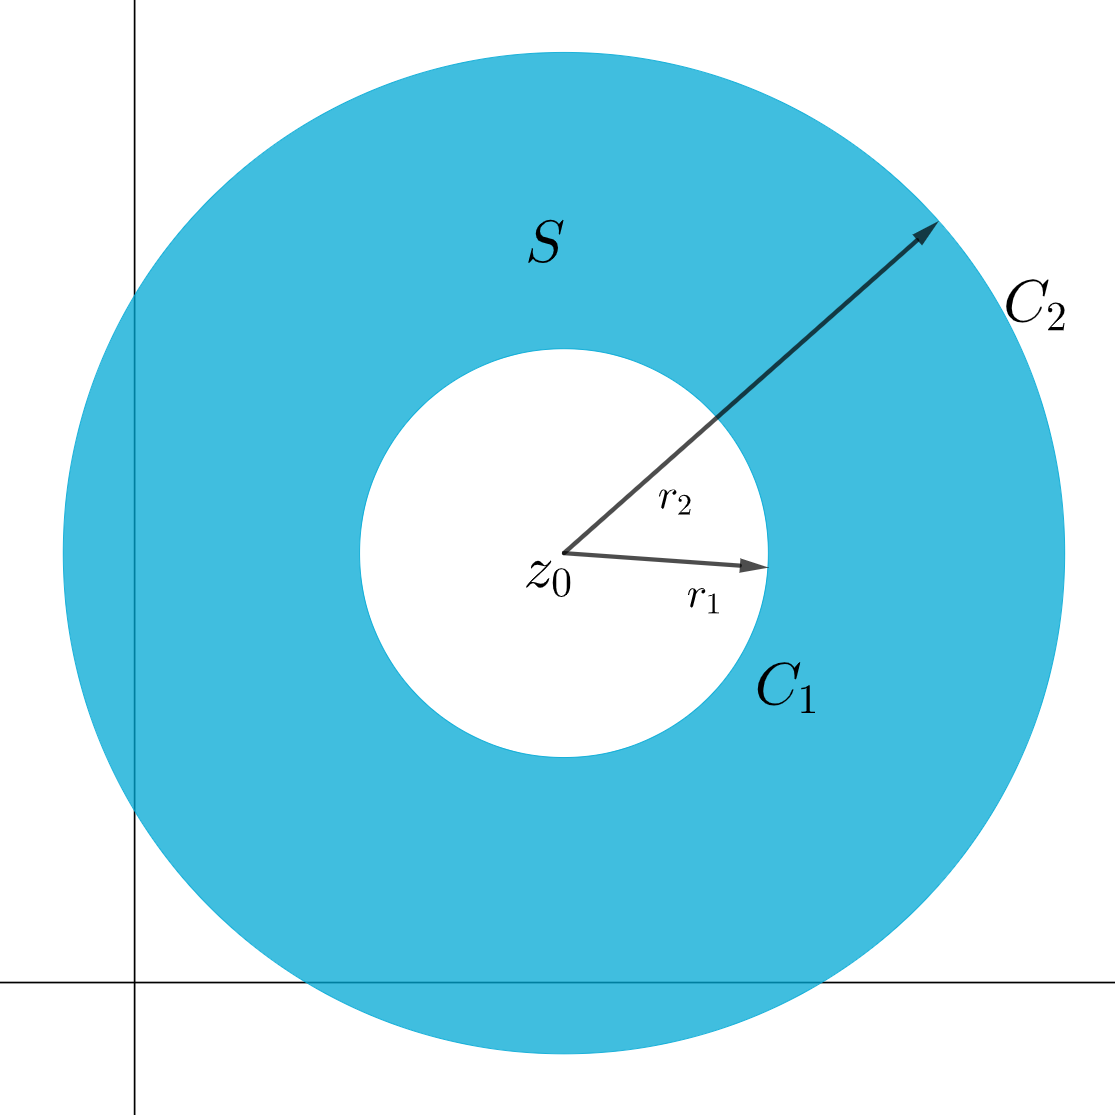
\includegraphics[width=0.5\textwidth]{AnnularRegion.png}
            \caption{展开为$Laurent$级数的函数解析区域}
            \label{fig:Laurent_series}
        \end{figure}
        \begin{definition}[Laurent级数]\label{def:laurent_series}
            如图\ref{fig:Laurent_series}所示,设$f(z)$在圆环$S$内单值解析,$z$为$S$内任一点,则函数$f(z)$可以展开为幂级数形式.
            \begin{align*}
                f(z)=\sum_{n=-\infty}^{\infty}a_n(z-z_0)^n,\quad a_n=\frac{1}{2\pi i}\oint_{C}\frac{f(\xi)}{(\xi-z_0)^{n+1}}d\xi
            \end{align*}
        \end{definition}
        函数$f(z)$在内圆$C_1$内不解析,但注意$f(z)$在点$z_0$上可能解析也可能不解析.

        $Laurent$级数有两部分,其中正幂项在外圆$C_2$内内闭一致收敛,负幂项在内圆$C_1$外绝对收敛.其中负幂项被称为$Laurent$级数的主要部分,当$Laurent$级数没有
        负幂项时,它就是$Taylor$级数.


    \subsection{Laurent级数的计算}
        废话不多说,直接上例题.
        \begin{example}
            将函数$f(z)=\dfrac{2+3z}{z^2+z^3}$在$z=0$点处写成$Laurent$级数的形式.
        \end{example}
        \begin{solution}
            我们有:
            \begin{align*}
                f(z)&=\frac{1}{z^2}\left(\frac{2+3z}{1+z}\right)=\frac{1}{z^2}\left(3-\frac{1}{1+z}\right)
                =\frac{1}{z^2}\left(3-\sum_{n=0}^{\infty}(-1)^nz^n\right)\\
                &=\frac{1}{z^2}(3-1+z-z^2+z^3-\cdots)=\frac{2}{z^2}+\frac{1}{z}-1+z-z^2+\cdots
            \end{align*}
            该级数在$|z|<1$上收敛.
        \end{solution}

        \begin{example}
            讨论函数$f(z)=1/(4z-z^2)$的$Laurent$展开.
        \end{example}
        \begin{solution}
            该函数有两个奇点$z=0,\,z=4$.所以我们将该函数分别在$z=0$处和$z=\infty$处展开.

            当$|z|<4$时,我们有$|z/4|<1$:
            \begin{align*}
                f(z)=\frac{1}{4z}\left(\frac{1}{1-z/4}\right)=\frac{1}{4z}\sum_{n=0}^{\infty}\left(\frac{z}{4}\right)^n=\sum_{n=0}^{\infty}4^{-n-1}z^{n-1}=\sum_{n=-1}^{\infty}4^{-n-2}z^n.
            \end{align*}

            当$|z|>4$时,我们有$|4/z|>1$(此时是在点$z=\infty$处展开):
            \begin{align*}
                f(z)=-\frac{1}{z^2}\left(\frac{1}{1-4/z}\right)=-\frac{1}{z^2}\sum_{n=0}^{\infty}4^nz^{-n}=-\sum_{-\infty}^{-2}4^{-n-2}z^{n}.
            \end{align*}
        \end{solution}

        从上面这俩例题我们能看到求解$Laurent$级数和使用间接法求解$Taylor$级数十分类似,只是需要注意自变量的取值范围.

    \subsection{奇点的分类}
        定义\ref{def:singular_point}将奇点定义为函数$f$不解析的点,实际上奇点还可以细分为
        在其任一空心邻域上均解析的孤立奇点和在其任一空心邻域上都有其他奇点的非孤立奇点.
        孤立奇点根据函数的$Laurent$级数又可以分为可去奇点、极点和本性奇点.

        \begin{remark}
            非孤立奇点一般出现在多值函数中.
        \end{remark}

        \begin{enumerate}
            \item 可去奇点\\
                级数展开式不含负幂项.$f(z)=\sum_{n=0}^{\infty}a_n(z-z_0)^n$
            \item 极点\\
                级数展开式含有有限个负幂项,特别的,如果级数展开式含有$m,\ (m\neq \infty)$个负幂项,则称为$m$阶极点.$f(z)=\sum_{n=-m}^{\infty}a_n(z-z_0)^n$
            \item 本性奇点\\
                级数展开式含有无穷个负幂项.$f(z)=\sum_{-\infty}^{\infty}a_n(z-z_0)^n$
        \end{enumerate}

        \begin{note}
            当我们讨论$f(z)$的无穷远点时,我们可以令$z=1/t$,此时点$t=0$的性质就是点$z=\infty$处的性质.
        \end{note}


\section{解析延拓}

    \subsection{解析延拓的定义}
        \begin{definition}[解析延拓]\label{def:analytic_continuation}
            设有函数$f_1,\,f_2:\mathbbm{C}\to\mathbbm{C}$,分别在区域$G_1,\,G_2$上解析,且$G_1\cap G_2=g\neq \varnothing$.如果有$\forall z\in g,\ f_1(z)\equiv f_2(z)$,
            则称$f_1$是$f_2$在$G_1$中的解析延拓,$f_2$是$f_1$在$G_2$中的解析延拓.
        \end{definition}

    \subsection{解析延拓的应用}
        使用复分析处理问题的时候,我们就可以先在较小区域内定义出复变函数,再使用解析延拓将其拓展到我们想要使用的地方,
        黎曼$\zeta $函数和$\Gamma$函数就是通过解析延拓得到的.我们的课程并没有详细讲解解析延拓,也不会考察,但是解析延拓在后续数学物理的学习中用处挺大,有兴趣很建议详细学习相关内容.
